\documentclass[letterpaper, 12pt]{article}

\usepackage{caption}
\usepackage[T1]{fontenc}
\usepackage[lmargin=1 in, rmargin=1 in, tmargin=1 in, bmargin=1 in]{geometry}
\usepackage{graphicx}
\usepackage{hyperref}
\usepackage{times}
\usepackage{xcolor}

\begin{document}

\begin{center}
\includegraphics[width=\textwidth, trim={5cm 0.5cm 7.5cm 1.5cm},clip]{figures/BH_PWS_PWS_0.eps}
\captionsetup{type=figure}
\captionof{figure}{Stacks of the envelopes of the cross correlation signals for different positions of the tremor source relative to the Burnt Hill array. See caption of Figure 4 for an explanation of this figure.}
\end{center}

\begin{center}
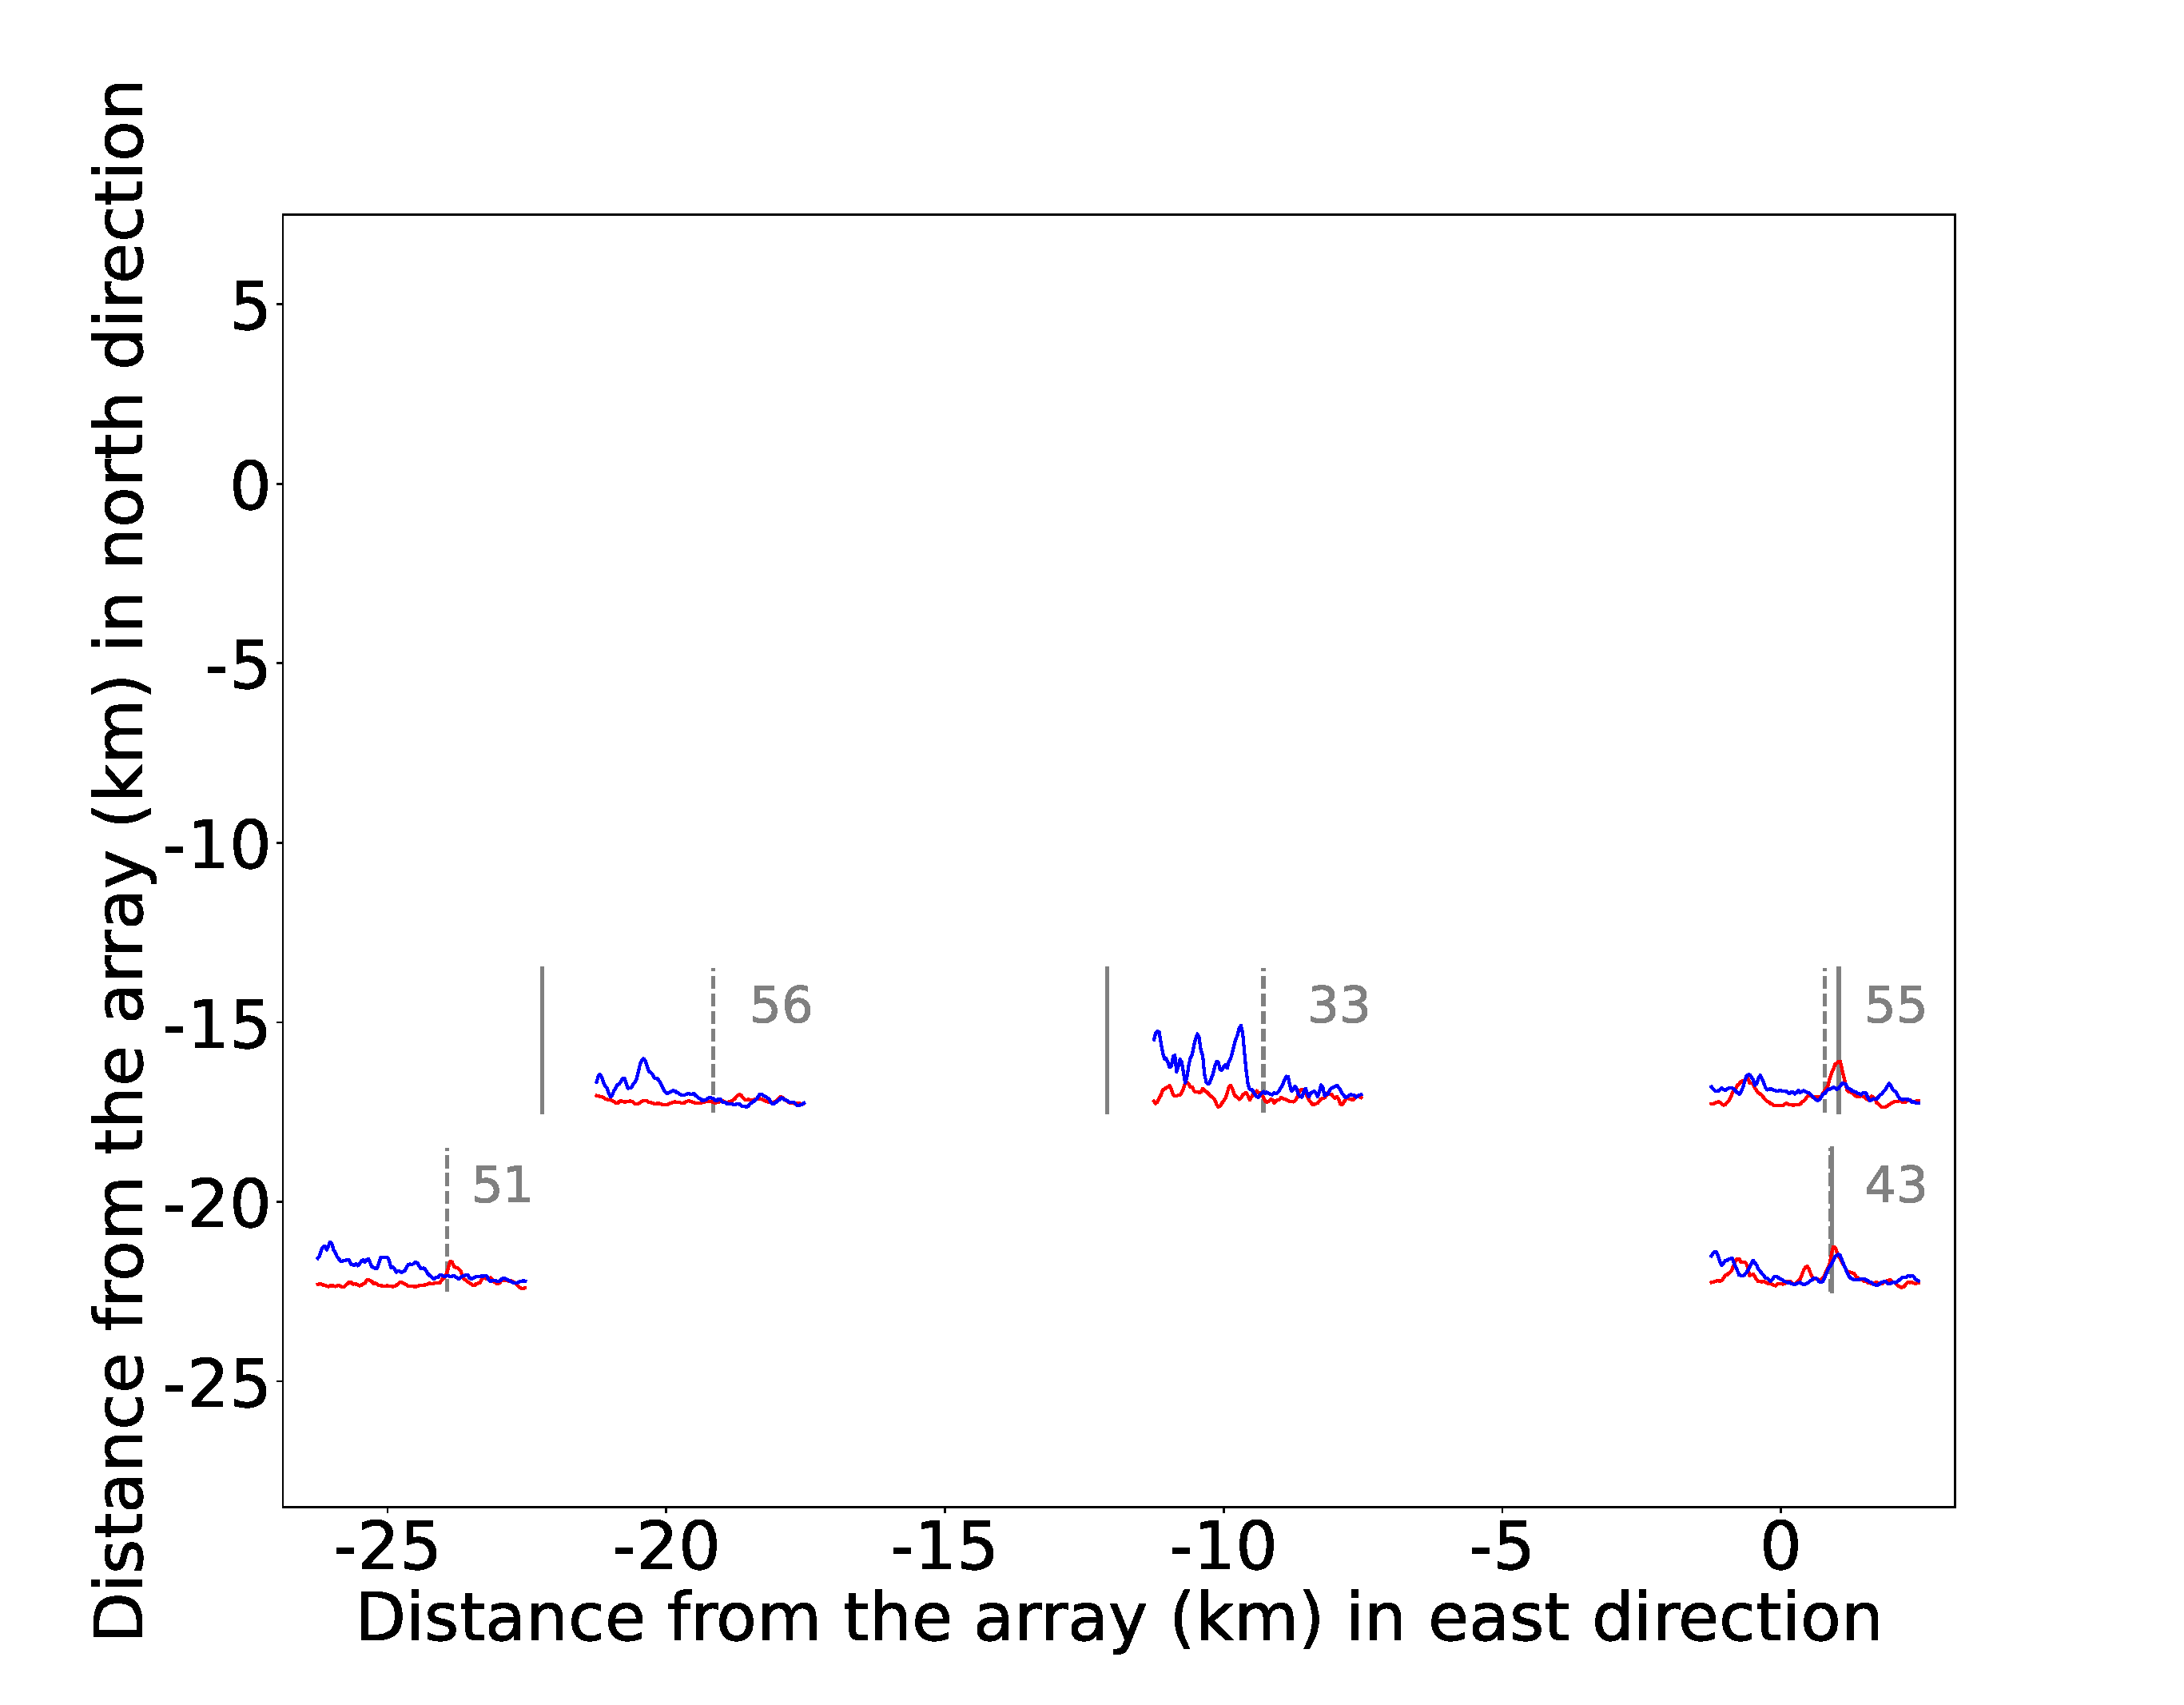
\includegraphics[width=\textwidth, trim={1.5cm 1cm 4.5cm 1.5cm},clip]{figures/CL_PWS_PWS_0.eps}
\captionsetup{type=figure}
\captionof{figure}{Stacks of the envelopes of the cross correlation signals for different positions of the tremor source relative to the Cat Lake array. See caption of Figure 4 for an explanation of this figure.}
\end{center}

\begin{center}
\includegraphics[width=\textwidth, trim={1cm 0.5cm 2.5cm 1.5cm},clip]{figures/DR_PWS_PWS_0.eps}
\captionsetup{type=figure}
\captionof{figure}{Stacks of the envelopes of the cross correlation signals for different positions of the tremor source relative to the Danz Ranch array. See caption of Figure 4 for an explanation of this figure.}
\end{center}

\begin{center}
\includegraphics[width=\textwidth, trim={1.5cm 1cm 4.5cm 4cm},clip]{figures/GC_PWS_PWS_0.eps}
\captionsetup{type=figure}
\captionof{figure}{Stacks of the envelopes of the cross correlation signals for different positions of the tremor source relative to the Gold Creek array. See caption of Figure 4 for an explanation of this figure.}
\end{center}

\begin{center}
\includegraphics[width=\textwidth, trim={1cm 0.5cm 2.5cm 1.5cm},clip]{figures/LC_PWS_PWS_0.eps}
\captionsetup{type=figure}
\captionof{figure}{Stacks of the envelopes of the cross correlation signals for different positions of the tremor source relative to the Lost Cause array. See caption of Figure 4 for an explanation of this figure.}
\end{center}

\begin{center}
\includegraphics[width=\textwidth, trim={1.5cm 0.5cm 4.5cm 1.5cm},clip]{figures/PA_PWS_PWS_0.eps}
\captionsetup{type=figure}
\captionof{figure}{Stacks of the envelopes of the cross correlation signals for different positions of the tremor source relative to the Port Angeles array. See caption of Figure 4 for an explanation of this figure.}
\end{center}

\begin{center}
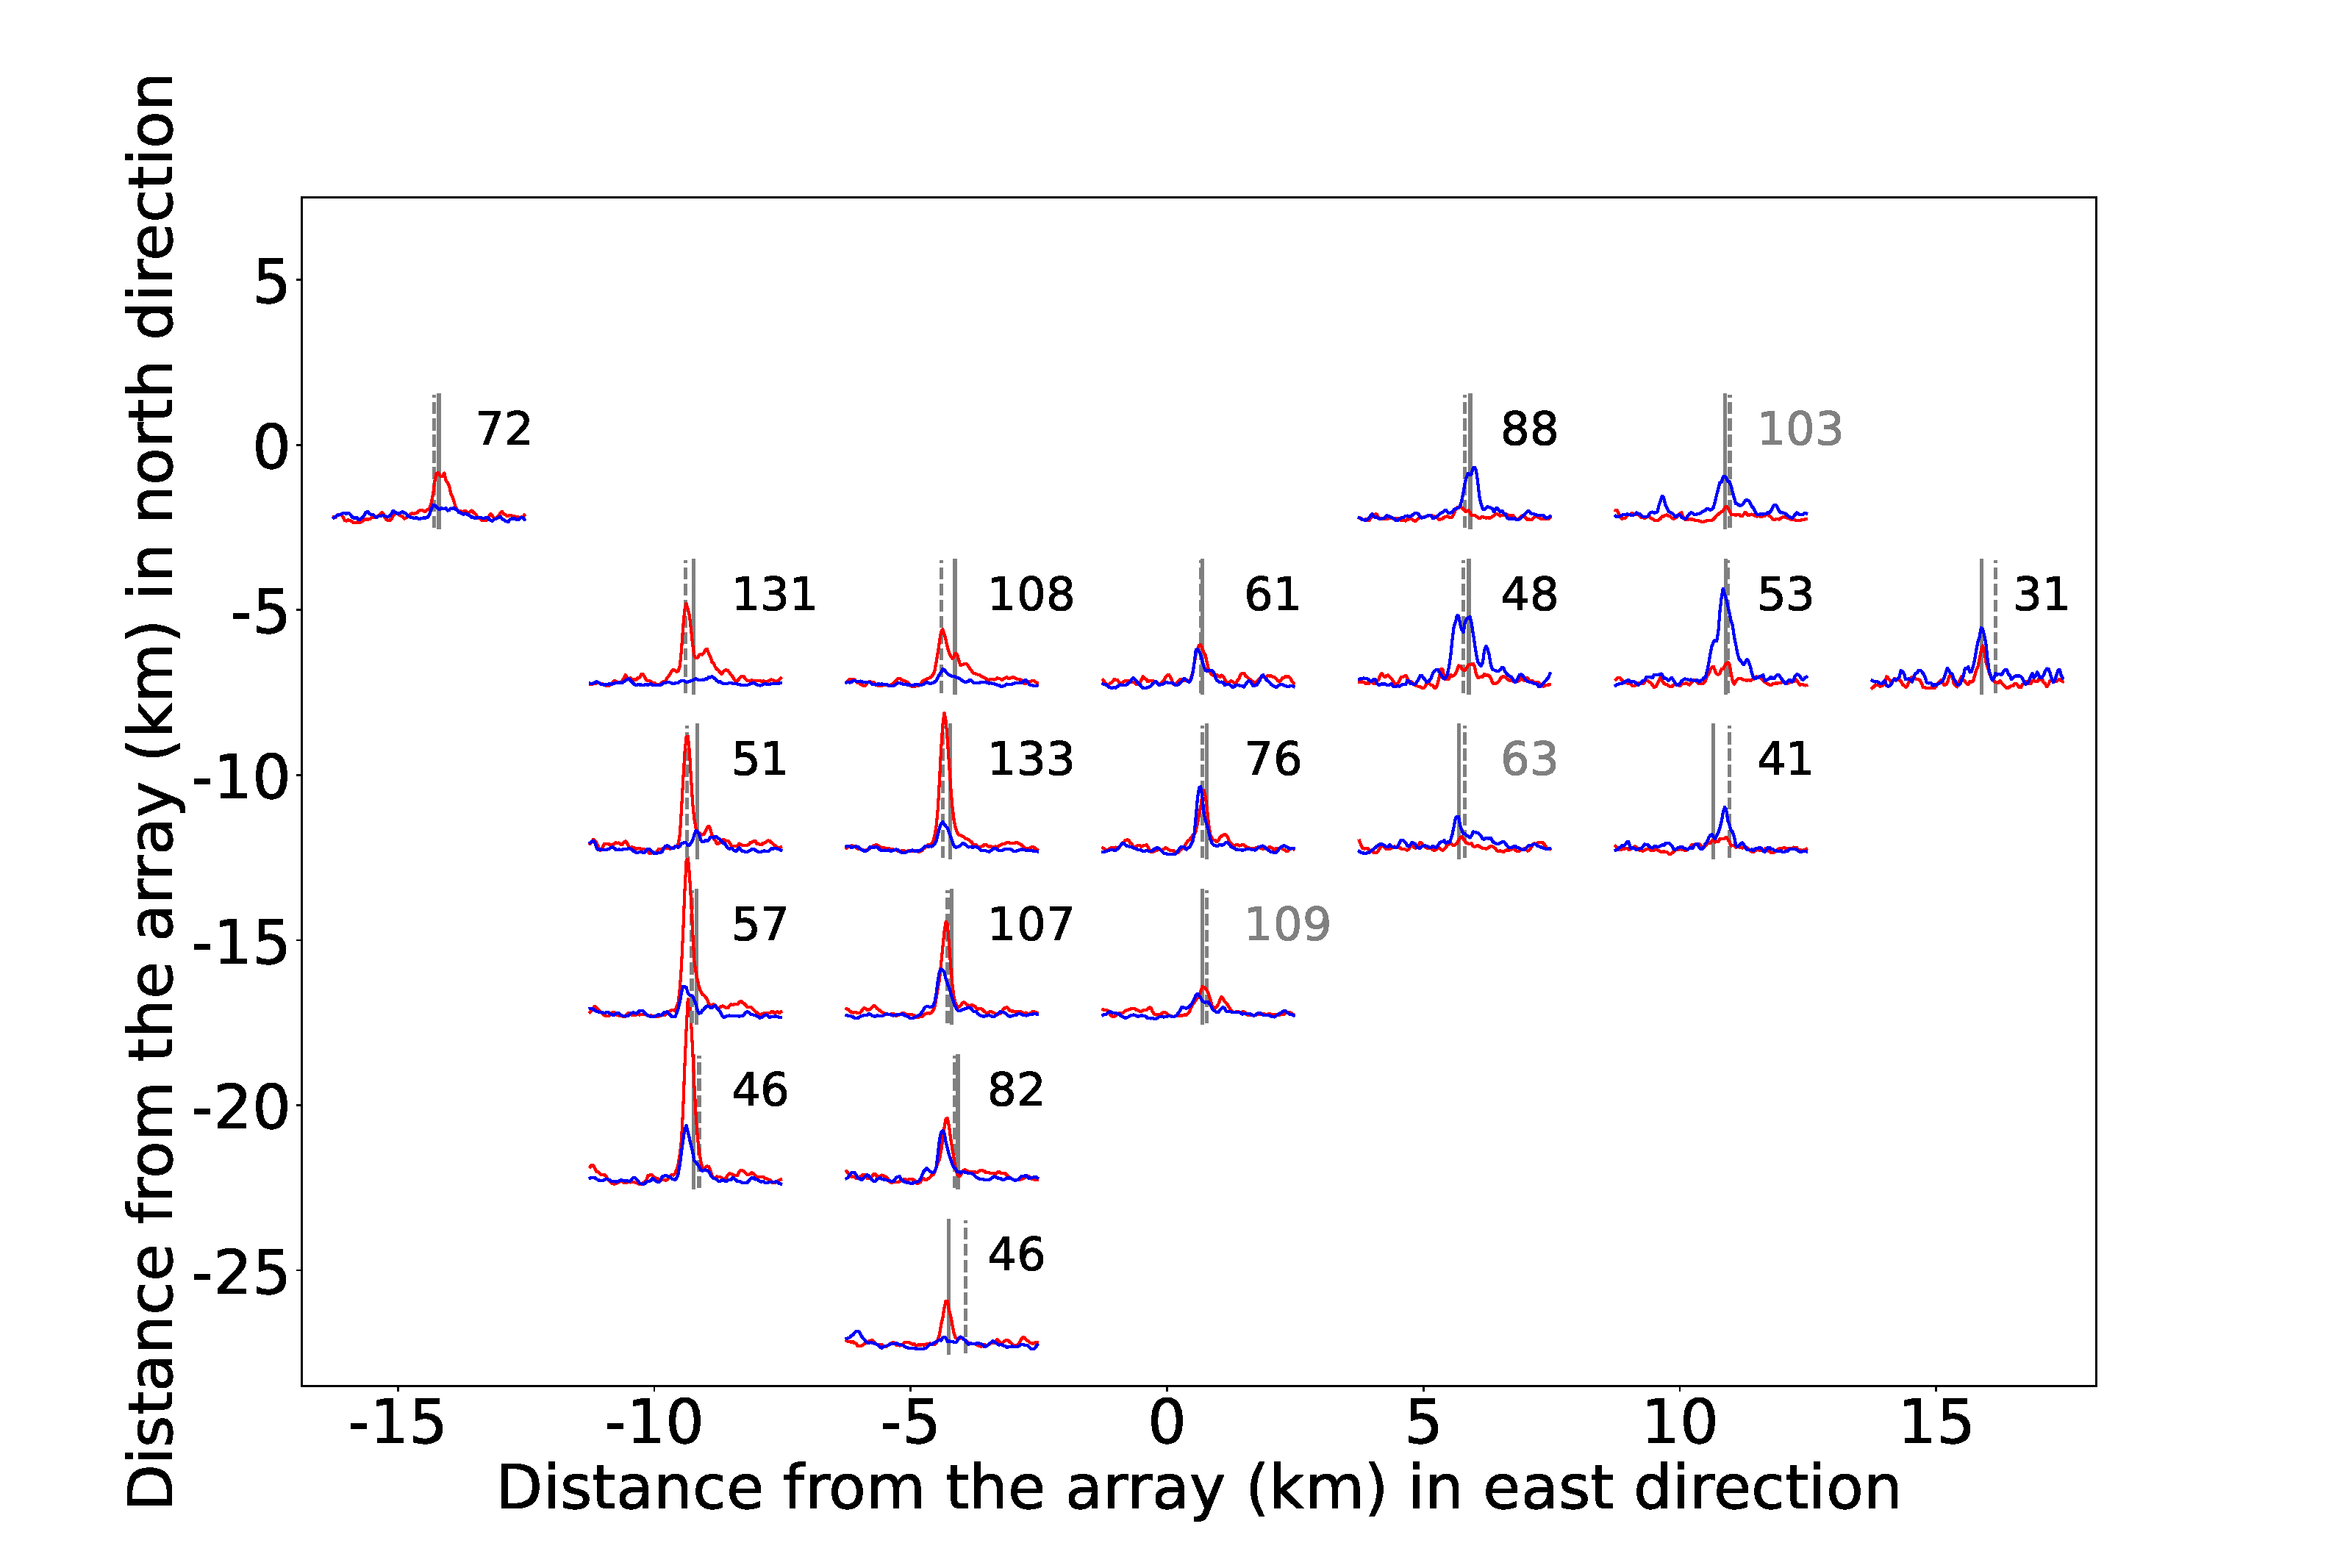
\includegraphics[width=\textwidth, trim={2.5cm 0.5cm 5cm 1.5cm},clip]{figures/TB_PWS_PWS_0.eps}
\captionsetup{type=figure}
\captionof{figure}{Stacks of the envelopes of the cross correlation signals for different positions of the tremor source relative to the Three Bumps array. See caption of Figure 4 for an explanation of this figure.}
\end{center}

\end{document}